\documentclass[notes=show]{beamer}

\usepackage{comment}
\usepackage{default}
\usepackage[utf8]{inputenc}
\usepackage{listings}
\usepackage{graphicx}

\graphicspath{{./images/}}

\definecolor{OliveGreen}{cmyk}{0.64,0,0.95,0.40}
\definecolor{Gray}{gray}{0.5}

\lstset{
    language=C,
    basicstyle=\ttfamily\scriptsize,
    keywordstyle=\color{OliveGreen},
    commentstyle=\color{Gray},
    captionpos=b,
    breaklines=true,
    breakatwhitespace=false,
    showspaces=false,
    showtabs=false,
    numbers=left,
}

\title{An Efficient Parallel Signal Temporal Logic Implementation}
\author{
	Bernhard Denner,
	Jakob Gruber,
	Mino Sharkhawy
}

\begin{document}

\maketitle

\begin{frame}
\frametitle{Signal Temporal Logic}
\begin{itemize}
    \item describing timed behaviours of continuous systems (time discrete signals)
    \item monitoring STL 
          \begin{itemize}
        	\item evaluate a satisfaction function of STL formula
        	\item boolean semantic
        	\item quantitative semantic, robustness of satisfation
          \end{itemize}
    \item based on
          \begin{itemize}
        	\item functions (like $\leq$ ), satisfaction of function
        	\item logical operators (NOT, AND, OR), combining satisfactions
        	\item temporal operators (UNTIL, EVENTUALLY, GLOBALLY), take timed behaviour into account
          \end{itemize}
\end{itemize}
% Very brief recap
\end{frame}

\begin{frame}
\frametitle{Objectives}
\begin{itemize}
	\item reimplement the robustness calculation operators with CUDA
	\begin{itemize}
	    \item based on algorithms presented in paper \emph{Efficient Robust Monitoring for STL} (A. Donze, T. Ferrere, O. Maler)
	    \item main task: find a efficient parallel solution for the operator implementation
	    \item very challenging for some operators
    \end{itemize}
	\item main goal: be much faster than the reference implementation (Breach)
	\item but always be as precise as the Breach
	\item if possible: integrate the CUDA implementation in MATLAB (Breach)
\end{itemize}
\end{frame}

\begin{frame}
\frametitle{Work Division}
\begin{itemize}
\item A lightweight on-the-fly plan
\item Organized through the bitbucket issue tracker
\item Jakob: Test suite, AND, UNTIL
\item Mino: EVTL, BEVTL
\item Bernhard: AND, Benchmark framework, Matlab integration
\end{itemize}
\end{frame}

\begin{frame}
\frametitle{Testing and Benchmarks}
\begin{itemize}
\item CTest: Integration into build system
\item Check: Test framework
\item One test suite per operator
\item Comparison against Breach results
\item Benchmark framework: compare performance against Breach
\begin{itemize}
	\item test with various signal sizes
	\item generated signals and random signals
\end{itemize}
\end{itemize}
\begin{figure}[H]
    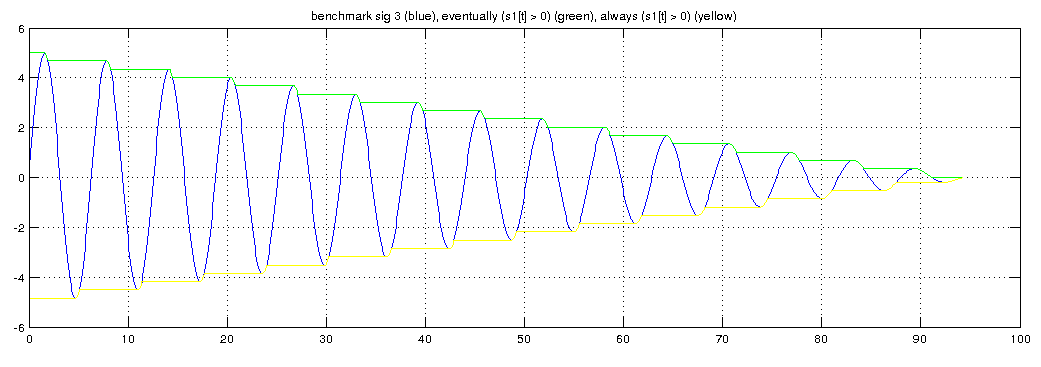
\includegraphics[scale=0.3]{bm_sig3_ev_alw.png}
\end{figure}
\end{frame}

\begin{frame}
\frametitle{Initial Plan}
% What did we initially want to do?
\begin{itemize}
\item Primitive operators
\begin{itemize}
\item NOT - done
\item AND - done
\item unbounded EVTL - done
\item unbounded UNTIL - partially done
\item bounded EVTL - done
\end{itemize}
\item Test suite - done
\item Benchmarking - done
\item Parser integration - not done
\item Optimization - not done
\end{itemize}
\end{frame}

\begin{frame}
\frametitle{Problems}
\begin{itemize}
\item Getting the breach reference implementation to work and to produce results for
        comparison was difficult.
\item Some operators very hard to parallelize
\begin{itemize}
\item Fully parallelized UNTIL needs infinite amount of memory
\item Even partial parallelization of UNTIL very difficult
\item Running time of parallel BEVTL depends on the window size
\end{itemize}
\item Floating point calculations very inaccurate, best accuracy: $5*10^{-5}$.
\end{itemize}
\end{frame}

\begin{frame}
\frametitle{Results}
\begin{itemize}
\item NOT trivially parallelizable
\item AND, EVTL involved, but possible in $O(f(n,p))$
\item UNTIL mostly possible, but one sequential part remains
\item BEVTL parallelizable, but dependent on window size $O(f(n,p,w))$
\end{itemize}
% Also, why we ended up with less than planned, what were the difficulties?
\end{frame}

\begin{frame}
\frametitle{Benchmarks - AND}
\begin{figure}[H]
    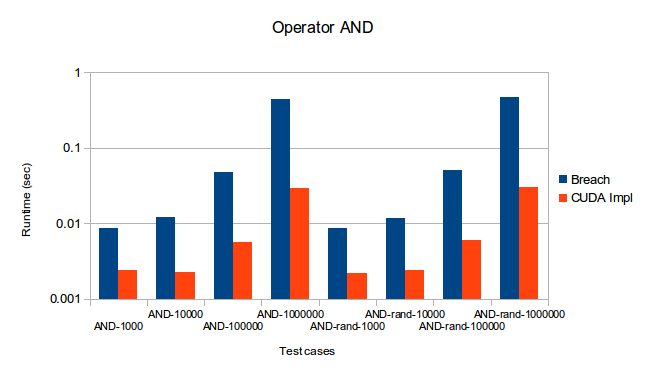
\includegraphics[scale=0.5]{bm_and.png}
    \caption{
        \label{fig:bm_and}
        Benchmark result: AND Operator}
\end{figure}
\end{frame}

\begin{frame}
\frametitle{Benchmarks - EVTL}
\begin{figure}[H]
    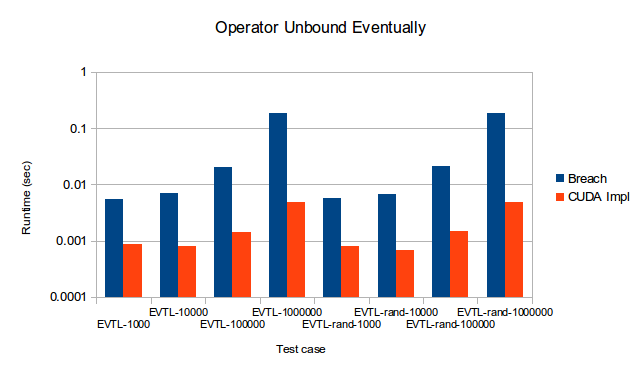
\includegraphics[scale=0.5]{bm_evtl.png}
    \caption{
        \label{fig:bm_evtl}
        Benchmark result: EVTL Operator}
\end{figure}
\end{frame}

\begin{frame}
\frametitle{Benchmarks - UNTIL}
\begin{figure}[H]
    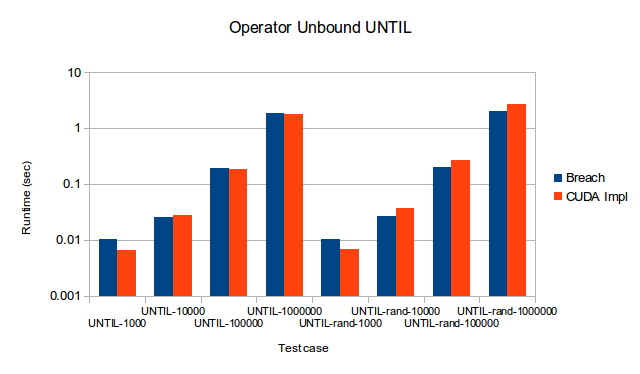
\includegraphics[scale=0.5]{bm_until.png}
    \caption{
        \label{fig:bm_until}
        Benchmark result: UNTIL Operator}
\end{figure}
\end{frame}

\begin{frame}
\frametitle{Benchmarks - BEVTL}
\begin{figure}[H]
    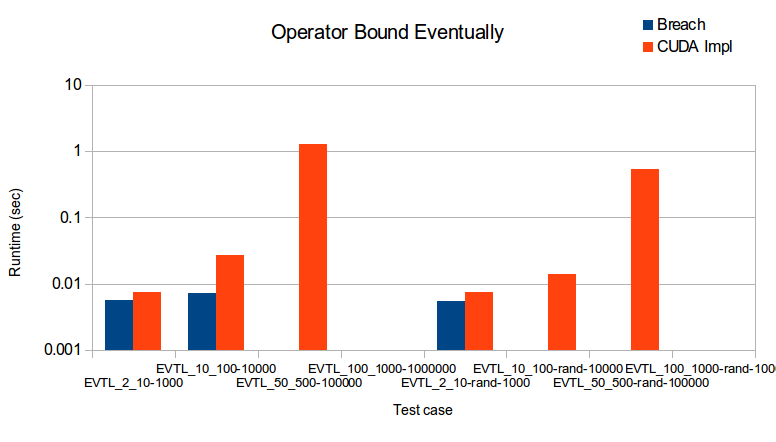
\includegraphics[scale=0.4]{bm_bevtl.png}
    \caption{
        \label{fig:bm_bevtl}
        Benchmark result: BEVTL Operator}
\end{figure}
\end{frame}

\begin{frame}
\frametitle{Lessons Learned}
\begin{itemize}
\item Create benchmarks at the beginning
\item Floating point arithmetic
\item Simple POC before implementation
\item Ensure task is possible before barging in
\end{itemize}
\end{frame}

\begin{frame}
\frametitle{Future Tasks}
\begin{itemize}
\item Completely parallel UNTIL, EVTL not dependent on window size
\item Multi-GPU
\item Optimizations
\item Processing entire formulas
\item Arbitrary expressions in input formulas
\end{itemize}
\end{frame}

\end{document}
